% 隔離テスト用ドライバ: 4-8 のみを単独ビルド（共有 main.tex には影響しない）
\documentclass[11pt,aspectratio=43,dvipsnames]{beamer}
\usepackage{luatexja}
\usepackage[match]{luatexja-fontspec}
\setmainjfont{HaranoAjiGothic}
\setsansjfont{HaranoAjiGothic}
\renewcommand{\kanjifamilydefault}{\gtdefault}
\usepackage{amsmath, amssymb}
\usepackage[version=4]{mhchem}
\usepackage{booktabs}
\usepackage{multirow}
\usepackage{colortbl}
\usepackage{graphicx}
\graphicspath{{figures/}}
\usepackage{pgfplots}
\pgfplotsset{compat=1.18}
% =====================================================================
%  seminar テーマ定義（既存 Marp デザインの Beamer 再現）
%  ・濃青の恒常ヘッダーバー（セクション名＋ページ番号）
%  ・専用表紙（アクセントライン＋グラデ背景）
%  ・本文は白地・濃青見出し
%  main.tex から \input する（パッケージではなく生プリアンブル）
% =====================================================================

% ---- ベース：装飾の少ないテーマから組む -----------------------------
\usetheme{default}
\usefonttheme{professionalfonts}
\setbeamertemplate{navigation symbols}{}   % ナビゲーション記号を消す

% ---- TikZ（ヘッダー・表紙・矢印などで使用）-------------------------
\usepackage{tikz}
\usetikzlibrary{arrows.meta, positioning, calc, shapes.geometric, fit, patterns}

% ---- 配色（ルール準拠）---------------------------------------------
\definecolor{HeaderBlue}{HTML}{0f5a7a}   % ヘッダー・見出しの濃青
\definecolor{DateGray}{HTML}{334b5e}     % 表紙の日付グレー
\definecolor{TitleBG}{HTML}{edf5fb}      % 表紙グラデの薄青

% コンテンツ用パレット（図・ハイライト・矢印で共通利用）
\definecolor{ArrowBlue}{HTML}{1F6FC4}    % 矢印・強調の青
\definecolor{HiPink}{HTML}{F4B6BE}       % ハイライト見出し（暖色）
\definecolor{HiBlue}{HTML}{C7DCEF}       % ハイライト見出し（寒色）
\definecolor{IpaBlue}{HTML}{1F5FC4}      % グラフ系列1（青）
\definecolor{DipeOrange}{HTML}{E8821E}   % グラフ系列2（橙）
\definecolor{SpRed}{HTML}{C0392B}        % 反応式：プロピレン強調の赤
\definecolor{SpBlue}{HTML}{1F6FC4}       % 反応式：エテン・エタン・CH0.5 の青

% 帯（ヘッダーバー）のパート別配色（寒色グラデ）。本文枠線は HeaderBlue のまま。
%  1-4 導入・全体像／5-9 反応・反応器／10-13 分離／14-17 最適化・経済・結言
\definecolor{barA}{HTML}{0F5A7A}   % 1-4  青緑
\definecolor{barB}{HTML}{1D6E6E}   % 5-9  シアン寄り
\definecolor{barC}{HTML}{2E4C8A}   % 10-13 青
\definecolor{barD}{HTML}{4A3C84}   % 14-17 紫

\setbeamercolor{normal text}{fg=black, bg=white}
\setbeamercolor{frametitle}{fg=HeaderBlue, bg=white}
\setbeamercolor{itemize item}{fg=HeaderBlue}
\setbeamercolor{itemize subitem}{fg=HeaderBlue}
\setbeamercolor{block title}{fg=white, bg=HeaderBlue}
\setbeamercolor{block body}{fg=black, bg=TitleBG}
\setbeamercolor{alerted text}{fg=HeaderBlue}

% ---- フォントサイズ（Marp px をおおよそ pt に対応）------------------
\setbeamerfont{frametitle}{size=\large, series=\bfseries}   % スライド見出し ~44px

% ---- 恒常ヘッダーバー（headline）-----------------------------------
%  左：セクション名（無ければロゴ枠）／右：ページ番号
\newcommand{\HeaderLogo}{}   % ロゴを入れるなら \renewcommand で画像指定
% 本線の総枚数（分母）。appendix に入ると分子がこれを超え、本線/付録を見分けられる。
\newcommand{\MainTotal}{17}
% パート別に帯色を選ぶ：1-4=barA／5-9=barB／10-13=barC／14-17=barD。
% スライド4の独自帯（CC・GCC）など headline を上書きする箇所でも呼べるよう独立コマンド化。
% 併せて本文アクセント色 HeaderBlue 自体をそのパート色へ再定義し、各スライドの
% 図・枠線・矢印・ボックス（HeaderBlue 参照）をパート色に連動させる（\colorlet は大域的）。
% headline はフレーム本文より前に組まれるため、ここでの再定義が本文に効く。
\newcommand{\SetBarColor}{%
  \ifnum\insertframenumber<5\setbeamercolor{headerbar}{fg=white, bg=barA}\colorlet{HeaderBlue}{barA}%
  \else\ifnum\insertframenumber<10\setbeamercolor{headerbar}{fg=white, bg=barB}\colorlet{HeaderBlue}{barB}%
  \else\ifnum\insertframenumber<14\setbeamercolor{headerbar}{fg=white, bg=barC}\colorlet{HeaderBlue}{barC}%
  \else\setbeamercolor{headerbar}{fg=white, bg=barD}\colorlet{HeaderBlue}{barD}%
  \fi\fi\fi}
\setbeamertemplate{headline}{%
  \ifnum\insertframenumber>0\relax
    \SetBarColor
    \begin{beamercolorbox}[wd=\paperwidth, ht=4.5ex, dp=1.8ex,
                           leftskip=1.2em, rightskip=1.2em]{headerbar}%
      \color{white}\bfseries\large
      \insertsectionhead%
      \hfill
      \insertframenumber/\MainTotal%
    \end{beamercolorbox}%
  \fi
}
\setbeamercolor{headerbar}{fg=white, bg=barA}
\setbeamertemplate{footline}{}             % フッターは使わない
\setbeamersize{text margin left=3mm, text margin right=3mm}  % 本文を横幅ぎりぎりまで

% 【必須ルール】帯と本文の間の余白を詰める（全スライド共通）。
%  beamer 既定の天井スキップで本文が帯から離れるのを、headline 直後の負スキップで打ち消す。
%  情報量最優先：無駄な上余白は作らない。各スライドは [t] 推奨。
\addtobeamertemplate{headline}{}{\vskip-2.6ex}

% frametitle はバーの直下に置く（左寄せ・濃青・太字）
\setbeamertemplate{frametitle}{%
  \vskip0.6ex
  \hspace{0.6em}\usebeamerfont{frametitle}\usebeamercolor[fg]{frametitle}\insertframetitle\par
  \vskip0.2ex
}

% ---- 箇条書きをシンプルに ------------------------------------------
\setbeamertemplate{itemize item}{\textbullet}
\setbeamertemplate{itemize subitem}{--}

% =====================================================================
%  再利用ヘルパー（どのスライドでも使える共通部品）
% =====================================================================
% 青い矢印 →（行中に置ける。結論や対応関係の明示に）
\newcommand{\bluearrow}{\tikz[baseline=-0.5ex]\draw[ArrowBlue, line width=1pt,
  -{Stealth[length=2.2mm]}] (0,0)--(0.55,0);}

% ハイライト見出し  \hilite{色}{テキスト}  例: \hilite{HiPink}{IPA選択率の温度依存性}
\newcommand{\hilite}[2]{\colorbox{#1}{\bfseries\normalsize #2}}

% パラメータ表  \paramtable{ 項目 & 値 \\ ... }  （左:項目 右:値、単位は数式推奨）
\newcommand{\paramtable}[1]{%
  {\footnotesize\renewcommand{\arraystretch}{1.15}%
   \begin{tabular}{@{\hspace{1em}}ll@{}}#1\end{tabular}}}

% =====================================================================
%  専用表紙コマンド  \seminartitlepage
%  ルール準拠：アクセントライン(120x8px相当) + 160度グラデ背景
%               h1 60px / h2 34px濃青 / 著者27px / 日付22pxグレー
%  使い方: \title{} \subtitle{} \author{} \date{} を設定後に呼ぶ
% =====================================================================
\newcommand{\seminartitlepage}{%
  \begin{frame}[plain]
    \begin{tikzpicture}[remember picture, overlay]
      % 背景グラデ（左上 薄青 → 右下 白、斜め）
      \shade[top color=TitleBG, bottom color=white, shading angle=20]
        (current page.south west) rectangle (current page.north east);
      % アクセントライン（上から少し下げて左に）
      \fill[HeaderBlue]
        ([xshift=9mm, yshift=-12mm]current page.north west)
        rectangle ++(16mm, 1.1mm);
      % テキストブロック（左寄せ・縦中央付近）
      \node[anchor=center, text width=0.86\paperwidth, align=center]
            at (current page.center) {%
        {\fontsize{22pt}{28pt}\selectfont\bfseries\color{black}\inserttitle\par}
        \vspace{0.3em}
        {\fontsize{16pt}{20pt}\selectfont\bfseries\color{HeaderBlue}\insertsubtitle\par}
        \vspace{1.0em}
        {\fontsize{13pt}{17pt}\selectfont\color{black}\insertauthor\par}
        \vspace{0.4em}
        {\fontsize{11pt}{14pt}\selectfont\color{DateGray}\insertdate\par}
      };
    \end{tikzpicture}
  \end{frame}
}

\setlength{\overfullrule}{6pt}
\begin{document}
\setcounter{framenumber}{3}
\section{反応工程}% =====================================================================
%  04  反応工程 — 反応ネットワーク・速度式・触媒失活
%  source_memo: 04_reaction.tex §4.2(反応ネットワークと速度式) /
%               §4.3.2-3(コーキングと活性低下 a(t,T))
%  失活グラフ実データ: pdh_simulator/src/catalyst_model.py _A_MATRIX
%               （要項§3-3 提供データ、温度400-700C × 時間0-30min）
%  方針：反応器モデル（支配方程式・Ergun）は載せない。
%        上=反応式と速度式／下左=触媒失活の要点／下右=a(t,T) グラフ。
%        色は反応式の化学種と、温度で意味を持つグラフの系列のみ。
% =====================================================================
% 活性 a を緑の太字で統一表示するマクロ
\definecolor{ActGreen}{HTML}{1BC24A}
\providecommand{\actA}{}\renewcommand{\actA}{{\color{ActGreen}\scalebox{1.2}{\ensuremath{\boldsymbol{a}}}}}
\begin{frame}

  % ===== 上：反応ネットワーク + 速度式（全幅）======================
  {\normalsize
   \renewcommand{\arraystretch}{1.18}%
   \begin{tabular}{@{}l@{\hspace{0.7em}}l@{\hspace{0.6em}}l@{}}
     {\scriptsize 脱水素}
       & \setlength{\fboxsep}{4pt}\setlength{\fboxrule}{1.2pt}%
         \fcolorbox{HeaderBlue}{white}{\boldmath$\mathrm{C_3H_8 \rightleftharpoons {\color{SpRed}C_3H_6} + H_2}$}
       & $\displaystyle r_1 = \actA\,k_1\frac{p_{\mathrm{C_3H_8}} - p_{\mathrm{C_3H_6}}p_{\mathrm{H_2}}/K_{\mathrm{eq}}}{1 + p_{\mathrm{C_3H_6}}/K_B}$ \\
     {\scriptsize クラッキング} & {\boldmath$\mathrm{C_3H_8 \rightarrow {\color{SpBlue}C_2H_4} + CH_4}$}
       & $\displaystyle r_2 = k_2\,p_{\mathrm{C_3H_8}}$ \\
     {\scriptsize 水素化} & {\boldmath$\mathrm{{\color{SpBlue}C_2H_4} + H_2 \rightarrow {\color{SpBlue}C_2H_6}}$}
       & $\displaystyle r_3 = k_3\,p_{\mathrm{C_2H_4}}p_{\mathrm{H_2}}$ \\
     {\scriptsize コーキング} & {\boldmath$\mathrm{{\color{SpRed}C_3H_6} \rightarrow 3\,{\color{SpBlue}CH_{0.5}} + 2.25\,H_2}$}
       & {\scriptsize 物質収支では微量・触媒を失活} \\
   \end{tabular}}

  \vspace{0.1em}
  {\scriptsize 速度定数は修正アレニウス、基準 $T_0=793\,\mathrm{K}$。$K_B$ はプロピレン吸着で高転化時 $r_1$ を抑制。}

  \vspace{0.15em}

  % ===== 下：触媒失活の要点（左）と a(t,T) グラフ（右）============
  \begin{columns}[T,onlytextwidth]
    \begin{column}{0.38\textwidth}
      {\bfseries 触媒失活}\par
      \vspace{0.3em}
      {\footnotesize\raggedright
        コークが活性点を被覆し触媒を失活\par
        活性 $\actA(t,T)$ は主反応のみに作用\par
        \quad $\to$\,\textbf{$r_{1,\mathrm{eff}}=\actA\,r_1$}\par
        \vspace{0.4em}
        高温ほど分オーダーで急速に失活\par
        運転温度では数分で大きく低下\par
        \quad $\to$\,\textbf{短周期の再生が不可欠}\par
      }
    \end{column}
    \begin{column}{0.62\textwidth}
      \centering
      \begin{tikzpicture}
        \begin{axis}[
          font=\scriptsize,
          width=0.99\linewidth, height=4.85cm,
          xmin=0, xmax=30, ymin=0, ymax=1,
          xtick={0,10,20,30}, ytick={0,0.2,0.4,0.6,0.8,1.0},
          xlabel={運転時間 [min]}, ylabel={活性 $\actA$},
          xlabel near ticks, ylabel near ticks,
          grid=both, major grid style={gray!18},
          tick align=outside, tickpos=left,
          legend style={font=\tiny, at={(0.99,0.99)}, anchor=north east,
                        draw=none, fill=white, fill opacity=0.82,
                        text opacity=1, inner sep=1.2pt, row sep=-3.2pt},
          legend columns=2, legend cell align=left,
          no markers, semithick,
        ]
          \addplot[blue]          coordinates {(0,1)(5,0.94)(10,0.90)(15,0.86)(20,0.84)(25,0.82)(30,0.81)}; \addlegendentry{$400\,^\circ$C}
          \addplot[cyan!70!blue]  coordinates {(0,1)(5,0.87)(10,0.80)(15,0.76)(20,0.72)(25,0.70)(30,0.68)}; \addlegendentry{$450\,^\circ$C}
          \addplot[teal]          coordinates {(0,1)(5,0.80)(10,0.68)(15,0.622)(20,0.57)(25,0.52)(30,0.49)}; \addlegendentry{$500\,^\circ$C}
          \addplot[olive]         coordinates {(0,1)(5,0.67)(10,0.52)(15,0.42)(20,0.36)(25,0.31)(30,0.28)}; \addlegendentry{$550\,^\circ$C}
          \addplot[orange]        coordinates {(0,1)(5,0.52)(10,0.35)(15,0.24)(20,0.18)(25,0.15)(30,0.13)}; \addlegendentry{$600\,^\circ$C}
          \addplot[red!70!black]  coordinates {(0,1)(5,0.38)(10,0.21)(15,0.13)(20,0.09)(25,0.07)(30,0.06)}; \addlegendentry{$650\,^\circ$C}
          \addplot[red]           coordinates {(0,1)(5,0.25)(10,0.12)(15,0.08)(20,0.06)(25,0.05)(30,0.04)}; \addlegendentry{$700\,^\circ$C}
        \end{axis}
      \end{tikzpicture}\par
      \vspace{0.1em}
      {\scriptsize 図　触媒活性 $\actA$ の経時低下、高温ほど急速に失活}
    \end{column}
  \end{columns}

  \vspace{0.05em}
  \par\noindent{\tiny (速度式パラメータ・活性データの出典：第17回プロセスデザイン学生コンテスト要項)}

\end{frame}

\section{反応器設計}% =====================================================================
%  05  反応器設計 — 結論＋採用構成（What & Why を一枚で）
%  source_memo: 04_reaction.tex §4.1 反応器形式の選定の3判断と結論、
%               §4.x 検証諸元 Table reactor_verification（trial #201）
%  方針：上=3つの設計判断を課題→対策で3列／下左=採用構成の模式図(TikZ)／
%        下右=キー諸元。色は状態(反応/再生)が意味を持つ模式図のみ。丸括弧禁止。
% =====================================================================
\begin{frame}

  % ===== 反応の性質 → 採用部品 の対応マップ ========================
  \vspace{0.2em}
  \centering
  \begin{tikzpicture}[
    >=Stealth, font=\footnotesize,
    prop/.style={draw=black!50, rounded corners=2pt, align=center,
                 inner sep=3pt, minimum height=0.62cm, text width=2.6cm},
    part/.style={draw=HeaderBlue, fill=HiBlue!45, rounded corners=2pt, align=center,
                 inner sep=3pt, minimum height=0.5cm, text width=3.5cm,
                 font=\footnotesize\bfseries},
    link/.style={-{Stealth[length=2mm]}, ArrowBlue, line width=1pt},
  ]
    % ---- 左：反応の性質 ----
    \node[prop] (heat) at (0,2.35) {吸熱};
    \node[prop] (eq)   at (0,1.15) {平衡支配\\高温・低圧 $0.5$ bar};
    \node[prop] (coke) at (0,0)    {コーキング\\数分で失活};
    % ---- 右：採用部品 ----
    \node[part] (hgm)   at (5.4,2.4) {床内 HGM 補温};
    \node[part] (shal)  at (5.4,1.6) {浅床軸流};
    \node[part] (multi) at (5.4,0.8) {多基・大断面・低速};
    \node[part] (swing) at (5.4,0.0) {スイング　反応 $\rightleftarrows$ 再生};
    % ---- 結線（どの性質がどの部品を強制するか）----
    \draw[link] (heat.east) -- (hgm.west);
    \draw[link] (eq.east)   -- (shal.west);
    \draw[link] (eq.east)   -- (multi.west);
    \draw[link] (coke.east) -- (swing.west);
    % ---- 見出し ----
    \node[font=\footnotesize\bfseries, anchor=south] at (0,2.85)   {反応の性質};
    \node[font=\footnotesize\bfseries, anchor=south] at (5.4,2.95) {採用部品};
  \end{tikzpicture}

  \vspace{0.05em}

  % ===== 下段：採用構成の模式図（左）／キー諸元（右）===============
  \begin{columns}[T,onlytextwidth]
    \begin{column}{0.58\textwidth}
      {\bfseries 採用構成　浅床軸流・多基並列スイング}\par
      \vspace{0.1em}
      \centering
      \scalebox{0.72}{%
      \begin{tikzpicture}[
        >=Stealth, font=\scriptsize,
        wall/.style={line width=1pt},
        proc/.style={-{Stealth[length=2mm]}, line width=1pt},
        flow/.style={-{Stealth[length=1.4mm]}, line width=0.5pt, black!65},
        dim/.style={{Stealth[length=1.6mm]}-{Stealth[length=1.6mm]}, line width=0.4pt},
        lead/.style={line width=0.3pt, black!55},
        lbl/.style={font=\scriptsize, align=left},
      ]
        \def\R{1.8}\def\Hb{1.35}\def\ry{0.62}
        % ---- 短胴・球形鏡板（扁平な大径容器）----
        \draw[wall] (-\R,0) -- (-\R,\Hb);
        \draw[wall] (\R,0) -- (\R,\Hb);
        \draw[wall] (-\R,\Hb) arc[start angle=180, end angle=0, x radius=\R, y radius=\ry];
        \draw[wall] (\R,0) arc[start angle=0, end angle=-180, x radius=\R, y radius=\ry];
        % ---- 入口ノズル（上）----
        \draw[wall] (-0.26,\Hb+\ry-0.02) -- (-0.26,\Hb+\ry+0.4);
        \draw[wall] (0.26,\Hb+\ry-0.02) -- (0.26,\Hb+\ry+0.4);
        \draw[wall] (-0.38,\Hb+\ry+0.4) rectangle (0.38,\Hb+\ry+0.5);
        \draw[proc] (0,\Hb+\ry+1.0) -- (0,\Hb+\ry+0.55);
        \node[lbl, anchor=west] at (0.45,\Hb+\ry+0.8) {原料ガス};
        % ---- 出口ノズル（下）----
        \draw[wall] (-0.26,-\ry+0.02) -- (-0.26,-\ry-0.4);
        \draw[wall] (0.26,-\ry+0.02) -- (0.26,-\ry-0.4);
        \draw[wall] (-0.38,-\ry-0.5) rectangle (0.38,-\ry-0.4);
        \draw[proc] (0,-\ry-0.55) -- (0,-\ry-1.0);
        \node[lbl, anchor=west] at (0.45,-\ry-0.8) {生成ガス};
        % ---- 分配板（多孔板）----
        \draw[line width=0.8pt] (-\R+0.05,1.08) -- (\R-0.05,1.08);
        \foreach \x in {-1.4,-1.0,-0.6,-0.2,0.2,0.6,1.0,1.4}{\draw[line width=0.4pt] (\x,1.08) -- (\x,0.98);}
        % ---- 触媒・HGM 混合浅床 ----
        \fill[HiBlue] (-\R+0.05,0.6) rectangle (\R-0.05,0.93);
        \draw[black!45] (-\R+0.05,0.6) rectangle (\R-0.05,0.93);
        % ---- 支持グリッド ----
        \draw[line width=0.8pt] (-\R+0.05,0.55) -- (\R-0.05,0.55);
        % ---- 床内 軸流（下向き）----
        \foreach \x in {-1.1,0,1.1}{\draw[flow] (\x,0.96) -- (\x,0.57);}
        % ---- 左ラベル ----
        \node[lbl, anchor=east] (ld) at (-\R-0.45,1.08) {分配板}; \draw[lead] (ld.east) -- (-\R+0.05,1.08);
        \node[lbl, anchor=east] (lc) at (-\R-0.45,0.77) {触媒・HGM 床}; \draw[lead] (lc.east) -- (-\R+0.05,0.77);
        \node[lbl, anchor=east] (lg) at (-\R-0.45,0.5) {支持グリッド}; \draw[lead] (lg.east) -- (-\R+0.05,0.55);
        % ---- 寸法 ----
        \draw[dim] (-\R,-1.2) -- (\R,-1.2); \node[below] at (0,-1.22) {$D$};
        \draw[dim] (\R+0.32,0.6) -- (\R+0.32,0.93); \node[right] at (\R+0.38,0.765) {$L_{\mathrm{bed}}$};
      \end{tikzpicture}}\par
      \vspace{0.1em}
      {\scriptsize 1 基の断面　$L_{\mathrm{bed}}\!\ll\! D$、常時 $7$／全 $14$ 基}\par
    \end{column}
    \begin{column}{0.42\textwidth}
      % 諸元は最良設計点 trial #201（スライドには番号を出さない）
      {\bfseries キー諸元}\par
      \vspace{0.4em}
      {\setlength{\fboxsep}{5pt}\setlength{\fboxrule}{1pt}%
       \fcolorbox{HeaderBlue}{white}{%
        \footnotesize\renewcommand{\arraystretch}{1.08}%
        \begin{tabular}{@{}l@{\hspace{1em}}l@{}}
          総基数 $N_{\mathrm{total}}$        & $14$ 基 \\
          並列基数 $N_{\mathrm{online}}$      & $7$ \\
          浅床厚 $L_{\mathrm{bed}}$           & $1.58$ m \\
          触媒粒径 $d_p$                      & $5.84$ mm \\
          入口温度 $T_{\mathrm{in}}$          & $935$ K \\
          床温降下 $\Delta T_{\max}$          & $50$ K \\
          有効触媒分率 $\phi_{\mathrm{cat}}$  & $0.85$ \\
          HGM 補償熱 $Q_{\mathrm{HGM}}$       & $24.96$ MW \\
        \end{tabular}}}
    \end{column}
  \end{columns}

\end{frame}

\section{支配方程式}% =====================================================================
%  06  支配方程式（ヘッダー＝支配方程式）
%  source_memo: 04_reaction.tex §4.2.4 支配方程式（物質・エネルギー・Ergun）/
%               §4.2.4 前提の粒内拡散検証 Weisz-Prater Φ・有効係数 η /
%               §4.2 量論行列(eq:stoich_matrix)・成分ベクトル
%  方針：見出しは置かない。速度式は §反応工程(スライド4)で既出のため載せない。
%        左＝支配方程式3本＋粒内拡散の検証式（反応律速の根拠）。
%        右＝記号を全集約：ベクトル/行列の成分＋スカラー記号の凡例。色なし・丸括弧禁止。
% =====================================================================
\begin{frame}[t]

  \vspace{0.4em}

  \begin{columns}[T,onlytextwidth]
    % ===== 左：支配方程式（3本）＋粒内拡散の検証 ====================
    \begin{column}{0.55\textwidth}
      {\footnotesize 組成（物質収支）}\par
      {\centering$\displaystyle\frac{d\boldsymbol{F}}{dz}=(1-\varepsilon)\,A_{\mathrm{cross}}\,\boldsymbol{\nu}\,\boldsymbol{r}$\par}
      \vspace{1.7em}
      {\footnotesize 温度（エネルギー収支・断熱）}\par
      {\centering$\displaystyle\frac{dT}{dz}=-\frac{(1-\varepsilon)\,A_{\mathrm{cross}}\,\boldsymbol{\Delta H}^{\!\top}\boldsymbol{r}}{\boldsymbol{F}^{\!\top}\boldsymbol{C}_p}$\par}
      \vspace{1.7em}
      {\footnotesize 圧力（Ergun）}\par
      {\centering\resizebox{\linewidth}{!}{$\displaystyle\frac{dP}{dz}=-\Big[\,150\frac{(1-\varepsilon_b)^2\mu u}{\varepsilon_b^3(\phi d_p)^2}
           +1.75\frac{(1-\varepsilon_b)\rho u^2}{\varepsilon_b^3\phi d_p}\,\Big]$}\par}
      \vspace{1.7em}
      {\footnotesize 粒内拡散の検証（Weisz--Prater）}\par
      {\centering\resizebox{0.9\linewidth}{!}{$\displaystyle\Phi=\frac{r_{\mathrm{obs}}R_p^2}{D_e\,C_s}\approx 0.22<0.3,
           \qquad D_e=\frac{\varepsilon_p}{\tau}\,D_{\mathrm{mol}}$}\par}
      \vspace{0.5em}
      {\footnotesize\centering $\Rightarrow\ \eta\approx 1$ となり反応律速が妥当\par}
    \end{column}

    % ===== 右：記号を全集約（ベクトル・行列＋スカラー凡例）=========
    \begin{column}{0.45\textwidth}
      {\centering\resizebox{\linewidth}{!}{%
        $\boldsymbol{F}=(F_{\mathrm{C_3H_8}},F_{\mathrm{C_3H_6}},F_{\mathrm{H_2}},F_{\mathrm{C_2H_4}},F_{\mathrm{CH_4}},F_{\mathrm{C_2H_6}})^{\!\top}$}\par}
      \vspace{0.4em}
      {\centering$\boldsymbol{r}=(r_1,r_2,r_3)^{\!\top}$\par}
      \vspace{0.35em}
      {\centering$\boldsymbol{\Delta H}=(\Delta H_1,\Delta H_2,\Delta H_3)^{\!\top}$\par}
      \vspace{0.5em}
      {\centering$\displaystyle
        \boldsymbol{\nu}=
        \begin{pmatrix}
          -1 & -1 &  0 \\
           1 &  0 &  0 \\
           1 &  0 & -1 \\
           0 &  1 & -1 \\
           0 &  1 &  0 \\
           0 &  0 &  1
        \end{pmatrix}
        \begin{matrix}
          \scriptstyle\mathrm{C_3H_8}\\[1pt]\scriptstyle\mathrm{C_3H_6}\\[1pt]\scriptstyle\mathrm{H_2}\\[1pt]
          \scriptstyle\mathrm{C_2H_4}\\[1pt]\scriptstyle\mathrm{CH_4}\\[1pt]\scriptstyle\mathrm{C_2H_6}
        \end{matrix}$\par}
      \vspace{0.45em}
      {\centering\resizebox{0.9\linewidth}{!}{%
        $\boldsymbol{C}_p=(C_{p,\mathrm{C_3H_8}},\dots,C_{p,\mathrm{C_2H_6}})^{\!\top}$}\par}
      \vspace{0.55em}
      {\color{black!25}\rule{\linewidth}{0.4pt}}\par
      \vspace{0.35em}
      {\scriptsize\raggedright
       $z$ 軸方向位置・$\varepsilon$ 床/容器体積比・$A_{\mathrm{cross}}$ 断面積・
       $T,P$ 温度/全圧・$\varepsilon_b$ 粒子間空隙率・$u$ 空塔速度・
       $\rho$ 密度・$\mu$ 粘度・$d_p$ 粒径・$\phi$ 形状係数・
       $R_p$ 粒子半径・$D_e,D_{\mathrm{mol}}$ 有効/分子拡散・$\varepsilon_p$ 粒子空隙率・
       $\tau$ 屈曲度・$C_s$ 表面濃度・$r_{\mathrm{obs}}$ 観測速度・$\eta$ 有効係数\par}
    \end{column}
  \end{columns}

\end{frame}

\section{反応器比較}% =====================================================================
%  07  反応器比較 — 選定の定量根拠（3判断の対比）
%  source_memo: 04_reaction.tex §4.1 移動床/スイング・軸流深床/径方向流/
%               浅床軸流・段間再加熱/床内HGM、図 reactor_pdrop_axial_feasibility
%  方針：左=3判断の対比表（採用に○）、右=軸流深床の圧損成立性マップで
%        浅床化の必然性を定量的に示す。丸括弧禁止。
% =====================================================================
\begin{frame}

  \begin{columns}[T,onlytextwidth]
    % ===== 左：3つの判断の対比 ===================================
    \begin{column}{0.5\textwidth}
      {\bfseries 3つの判断と採用根拠}\par
      \vspace{0.6em}
      {\footnotesize\renewcommand{\arraystretch}{1.25}%
       \begin{tabular}{@{}l l c@{}}
         \toprule
         判断 & 候補 & 採否 \\
         \midrule
         \multirow{2}{*}{触媒再生}
            & 移動床            & $\times$ \\
            & 並列スイング固定床 & $\bigcirc$ \\
         \midrule
         \multirow{3}{*}{流通形式}
            & 軸流深床   & $\times$ \\
            & 径方向流   & $\triangle$ \\
            & 浅床軸流   & $\bigcirc$ \\
         \midrule
         \multirow{2}{*}{熱補償}
            & 段間再加熱 & $\times$ \\
            & 床内 HGM   & $\bigcirc$ \\
         \bottomrule
       \end{tabular}}\par
      \vspace{0.8em}
      {\scriptsize
       $\times$ 移動床は数日寿命を要し分単位失活に追従不可\par
       $\triangle$ 径方向流は可行だが機構が複雑\par
       $\bigcirc$ 浅床軸流は単純構造で圧損を解消}\par
    \end{column}

    % ===== 右：圧力で妥協できない→幾何で解く（圧損成立性マップ）===
    %  source: monitor/reactor_pressure_drop_and_geometry.ipynb
    %    ①0.5bar 平衡で必須（647C: 0.5bar 78% / 5bar 37%）
    %    ②軸流深床 2-6mm 全床長 ΔP過大 検証36点すべて不成立
    %    ③浅床L↓＋多基u↓で成立（trial #201: 床1.7/総3.3%・X40.6%）
    \begin{column}{0.5\textwidth}
      {\bfseries 圧力で妥協できない $\to$ 幾何で解く}\par
      \vspace{0.2em}
      {\footnotesize 低圧ほど平衡転化率が高く $0.5$ bar が必須\par
       \hspace{0.6em}$647\,^\circ$C で $0.5$ bar 約 $78$ \%、$5$ bar 約 $37$ \%}\par
      \vspace{0.35em}
      \centering
      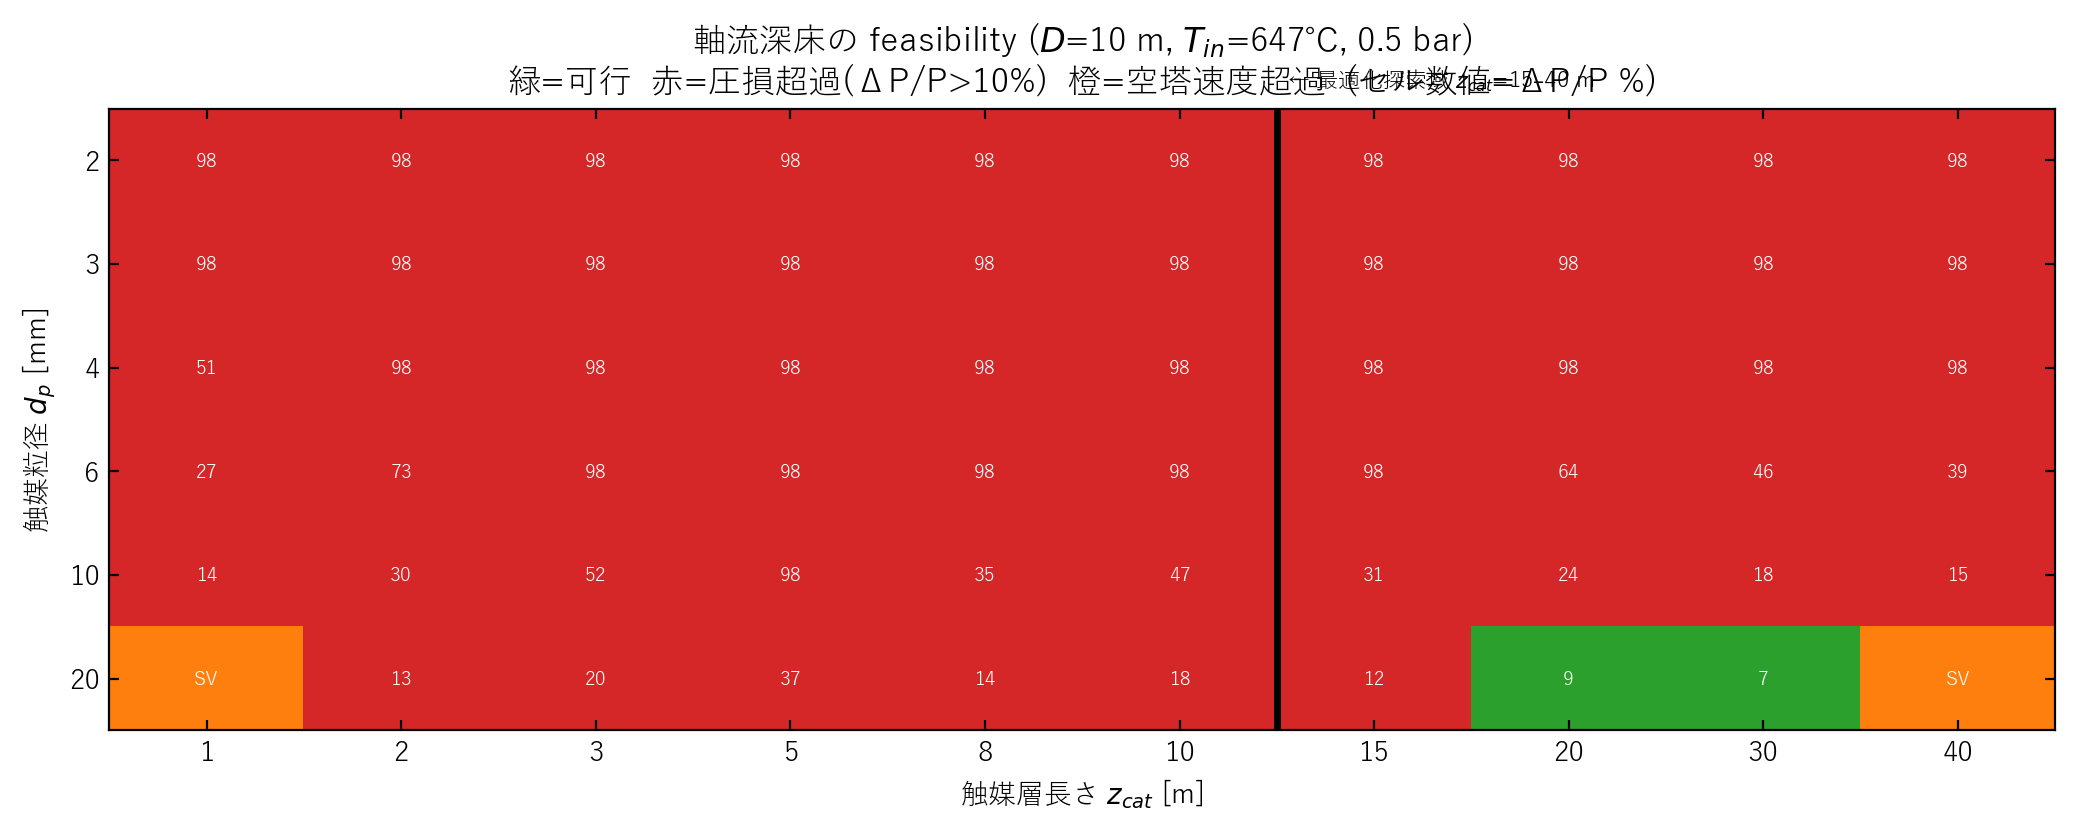
\includegraphics[width=\linewidth]{reactor_pdrop_axial_feasibility}\par
      \vspace{0.2em}
      {\scriptsize $D=10$ m・$0.5$ bar。現実粒径 $2\text{--}6$ mm の軸流深床は\par
       \hspace{0.6em}全床長で $\Delta P/P$ 過大、検証 $36$ 点すべて不成立}\par
      \vspace{0.3em}
      \raggedright
      {\footnotesize $\to$ \textbf{浅床で流路長↓・多基で流速↓}\par
       \hspace{0.6em}床/総 $\Delta P/P=1.7/3.3$ \%、転化率 $40.6$ \%}\par
    \end{column}
  \end{columns}

\end{frame}

\section{反応器プロファイル}% =====================================================================
%  08  反応器プロファイル — 炉内 軸方向挙動＋検証諸元
%  source_memo: monitor/reactor_axial_profile.ipynb 出力
%               reactor_axial_TX.png / reactor_axial_selectivity.png、
%               §4.x 検証諸元 Table reactor_verification（trial #201）
%  方針：左=軸方向プロファイル2図（T/X のHGM補償効果・選択率の床内崩落）、
%        右=検証諸元。丸括弧禁止。
% =====================================================================
\begin{frame}

  \begin{columns}[T,onlytextwidth]
    % ===== 左：軸方向プロファイル =================================
    \begin{column}{0.6\textwidth}
      {\bfseries HGM 補償が床温を維持し転化率を伸ばす}\par
      \vspace{0.1em}
      \centering
      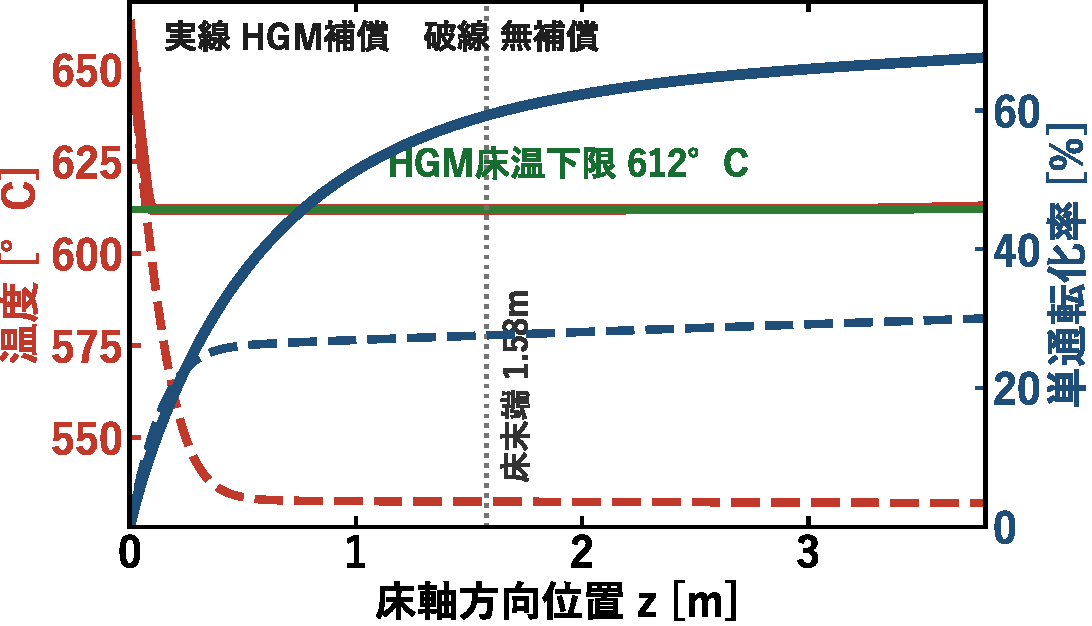
\includegraphics[width=0.78\linewidth]{reactor_axial_TX}\par
      \vspace{0.2em}
      {\bfseries 選択率は床後半で崩落し出口値へ収束}\par
      \vspace{0.1em}
      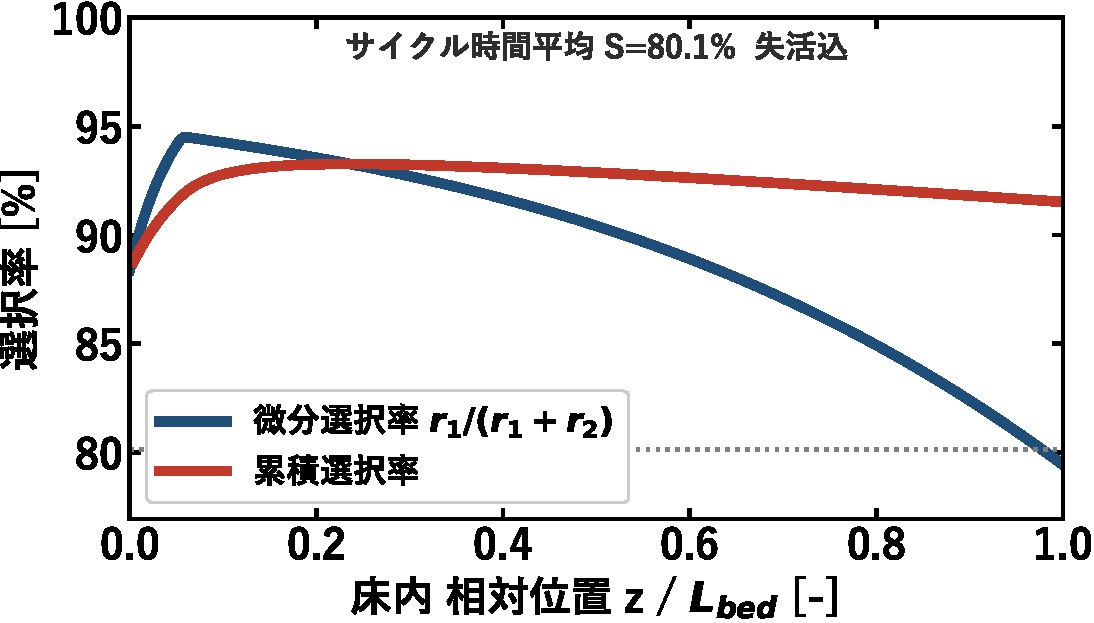
\includegraphics[width=0.78\linewidth]{reactor_axial_selectivity}\par
    \end{column}

    % ===== 右：検証諸元（trial #125）=============================
    \begin{column}{0.4\textwidth}
      {\bfseries 検証諸元　{\scriptsize 最良設計点}}\par
      \vspace{0.5em}
      {\setlength{\fboxsep}{5pt}\setlength{\fboxrule}{1pt}%
       \fcolorbox{HeaderBlue}{white}{%
        \footnotesize\renewcommand{\arraystretch}{1.25}%
        \begin{tabular}{@{}l@{\hspace{0.8em}}r@{}}
          入口温度 $T_{\mathrm{in}}$   & $935$ K \\
          出口温度 $T_{\mathrm{out}}$  & $885$ K \\
          床温降下 $\Delta T$          & $50$ K \\
          転化率 $X$                   & $40.6\,\%$ \\
          選択率 $S$                   & $80.1\,\%$ \\
          浅床厚 $L_{\mathrm{bed}}$    & $1.58$ m \\
          触媒粒径 $d_p$               & $5.84$ mm \\
          床 $\Delta P/P$              & $1.7\,\%$ \\
          総 $\Delta P/P$              & $3.3\,\%$ \\
          総基数 $N_{\mathrm{total}}$  & $14$ 基 \\
        \end{tabular}}}\par
      \vspace{0.8em}
      {\scriptsize 図の $T$・$X$ は新触媒断面、\par
       転化率 $40.6\,\%$・選択率 $80.1\,\%$ は\par
       失活を含むサイクル時間平均。\par
       無補償では床温が下限へ張り付き\par
       転化率が頭打ちとなる。}\par
    \end{column}
  \end{columns}

\end{frame}

\end{document}
